% "{'classe':('PSI'),'chapitre':'cin_geo','type':('application'),'titre':'Joint de cardan', 'source':'','comp':(''),'corrige':False}"
%\setchapterimage{fig_00.jpg}
\chapter*{Application \arabic{cptApplication} \\ 
Joint de cardan -- \ifprof Corrigé \else Sujet \fi}
\addcontentsline{toc}{section}{Application \arabic{cptApplication} : 
Joint de cardan -- \ifprof Corrigé \else Sujet \fi}

\iflivret \stepcounter{cptApplication} \else
\ifprof  \stepcounter{cptApplication} \else \fi
\fi

\setcounter{question}{0}

\marginnote[1cm]{
%\UPSTIcompetence[2]{B2-14}
%\UPSTIcompetence[2]{C1-05}
%\UPSTIcompetence[2]{C2-07}
}


\begin{marginfigure}
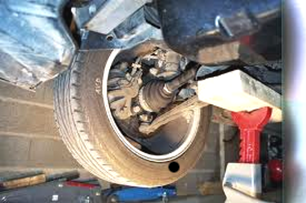
\includegraphics[width=\linewidth]{fig3_1}
\end{marginfigure}


\subsection*{Joint de Cardan}


Un joint de Cardan est un accouplement qui permet de transmettre un mouvement de rotation entre deux arbres concourants mais non alignés. L'angle maximum pratiquement utilisé entre les arbres est de $45\textdegree$. Une application courante est la transmission entre boite de vitesses  et roues-avant d’une voiture. 

Les vues ci-contre donnent des images d’un joint de cardan.

\begin{marginfigure}
%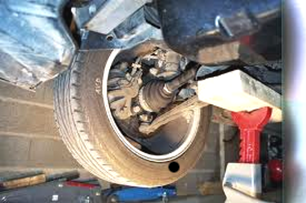
\includegraphics[width=.5\linewidth]{fig3_1}  

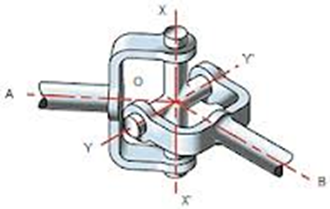
\includegraphics[width=\linewidth]{fig3_2}  

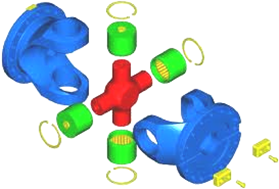
\includegraphics[width=\linewidth]{fig3_3} 
\end{marginfigure}

La modélisation suivante est proposée.
\begin{center}
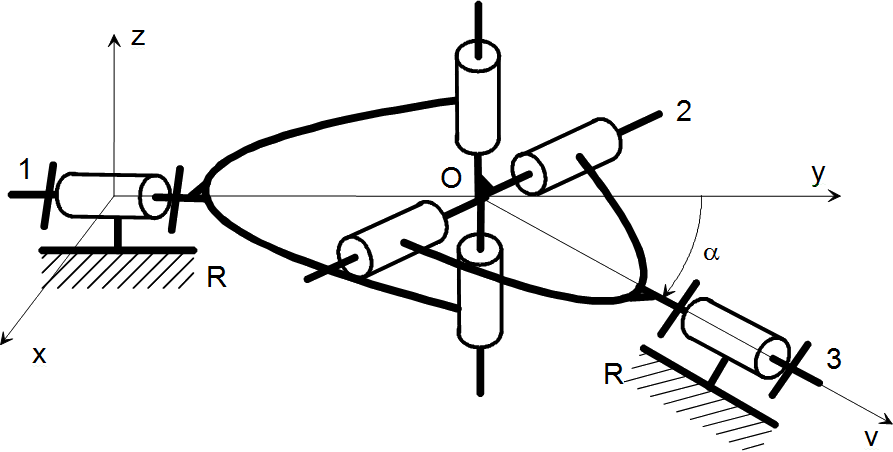
\includegraphics[width=.7\linewidth]{fig3_4} 
\end{center}

On appelle : 
\begin{itemize}
\item $\mathcal{R}$ le repère lié au solide $R$ considéré comme fixe. $\mathcal{R}=\left(O,\vect{x},\vect{y},\vect{z} \right)$;
\item $\mathcal{R}'$ le repère lié au solide R considéré comme fixe. $\mathcal{R}'=\left(O,\vect{u},\vect{v},\vect{z} \right)$. On pose $\alpha = \left(\vect{y},\vect{v} \right)$ (constant);
\item $\alpha$ l'"angle de brisure";
\item $\mathcal{R}_1$ le repère lié au solide 1. $\mathcal{R}_1 = \left(O,\vect{x_1},\vect{y},\vect{z_1} \right)$. On pose  $\theta_1 = \left(\vect{x},\vect{x_1} \right)$;
\item $\mathcal{R}_3$ le repère lié au solide 3. $\mathcal{R}_3 = \left(O,\vect{x_3},\vect{v},\vect{z_3} \right)$. On pose $\theta_3 = \left(\vect{u},\vect{x_3} \right)$.
\end{itemize}

\question{Tracer en vue orthogonale, les trois dessins (figures de changement de base) permettant le passage de $\mathcal{R}$ à $\mathcal{R}_1$ , de $\mathcal{R}$ à $\mathcal{R}'$ et de $\mathcal{R}'$ à $\mathcal{R}_3$.}
\ifprof
\begin{corrige}
\end{corrige}
\else\fi

\question{Exprimer la condition géométrique sur 2 permettant de lier $\mathcal{R}_1$ à $\mathcal{R}_3$.}
\ifprof
\begin{corrige}
\end{corrige}
\else\fi

\question{Développer cette relation et trouver la loi entrée sortie : $\theta_3 = f(\theta_1 , \alpha)$. Tracer, pour $\alpha=45\textdegree$, la courbe représentant l’évolution de la sortie $\theta_3$ en fonction de l’entrée $\theta_1$ avec $\theta_1$ variant de $-\pi$ à $+\pi$.}
\ifprof
\begin{corrige}
\end{corrige}
\else\fi

\question{Dériver cette relation par rapport au temps pour trouver la vitesse de sortie $\dot{\theta_3}$ en fonction de la vitesse d’entrée $\dot{\theta_1}$, de $\theta_1$ et de $\alpha$.}

\ifprof
\begin{corrige}
\end{corrige}
\else\fi


\ifprof
\else
\begin{marginfigure}
\centering

\includegraphics[width=3cm]{Cy_12_Ch_01_Application_02_Cardan_qr}
\end{marginfigure}
\fi

\question{Tracer l’évolution de la vitesse de sortie $\dot{\theta_3}$ en fonction notamment de l’évolution de l’angle d’entrée $\theta_1$. On prendra un angle de brisure de $45\textdegree$ et une vitesse d’entée constante $\dot{\theta_1}$ de 1 rad/s.}
\ifprof
\begin{corrige}
\end{corrige}
\else\fi

\question{Conclure sur une des propriétés de ce mécanisme.}
\ifprof
\begin{corrige}
\end{corrige}
\else\fi

